\newpage
\section{RESULTADOS}

Esta sección consolida los resultados experimentales obtenidos sobre la red de prueba de Stellar, conforme al
proceso de control de calidad definido en la metodología (pruebas unitarias, integración, antifraude y
medición). Los resultados se reportan en cuatro frentes: desempeño del contrato, cobertura de pruebas,
comportamiento antifraude y discusión comparativa.

\subsection{Metodología de medición}

Las métricas se capturan sobre testnet con el contrato \texttt{event\_contract} desplegado por el
\textit{factory} configurado para el prototipo. Las variables observadas son: tiempo de envío al RPC, tiempo
de confirmación on-chain (cierre del ledger que incluyó la transacción), latencia extremo a extremo desde la
interfaz hasta la actualización en la base de datos relacional, y tasa de fallos por tipo de operación. Cada
operación se ejecutó en corridas independientes y los percentiles se calculan sobre el conjunto observado.

\subsection{Desempeño sobre testnet}

La Tabla~\ref{tab:latencia} resume la latencia y el costo nominal por tipo de operación. El costo se reporta
en pesos colombianos (COP) calculados a la tasa de referencia promediada de 1\,XLM\,$\approx$\,1\,500\,COP.
Esta tasa es indicativa y está sujeta a la alta variabilidad del precio del activo en el mercado; la cifra
on-chain real es determinística en la unidad mínima de XLM.

\begin{table}[H]
\centering
\small
\renewcommand{\arraystretch}{1.3}
\definecolor{rowgray}{gray}{0.96}
\caption{Latencia de confirmación y costo nominal por operación sobre testnet.}
\label{tab:latencia}
\begin{tabularx}{\textwidth}{>{\raggedright\arraybackslash}p{4.0cm} >{\centering\arraybackslash}p{2.3cm}
>{\centering\arraybackslash}p{2.3cm} >{\centering\arraybackslash}p{2.3cm} >{\centering\arraybackslash}X}
\toprule
\rowcolor{rowgray}
\textbf{Operación} & \textbf{Envío (s)} & \textbf{Conf. p50 (s)} & \textbf{Conf. p95 (s)} & \textbf{Costo
aprox. (COP)} \\
\midrule
\texttt{crear\_boleto} & < 1 & 4{,}8 & 6{,}1 & $\approx$\,0{,}02 \\
\rowcolor{rowgray}
\texttt{listar\_boleto} & < 1 & 4{,}7 & 5{,}9 & $\approx$\,0{,}02 \\
\texttt{cancelar\_venta} & < 1 & 4{,}7 & 5{,}8 & $\approx$\,0{,}02 \\
\rowcolor{rowgray}
\texttt{comprar\_boleto} (primaria) & < 1 & 4{,}9 & 6{,}3 & $\approx$\,0{,}03 \\
\texttt{comprar\_boleto} (reventa) & < 1 & 5{,}1 & 6{,}5 & $\approx$\,0{,}06 \\
\rowcolor{rowgray}
\texttt{redimir\_boleto} & < 1 & 4{,}7 & 5{,}9 & $\approx$\,0{,}02 \\
\texttt{invalidar\_boleto} & < 1 & 4{,}8 & 6{,}0 & $\approx$\,0{,}02 \\
\bottomrule
\end{tabularx}
\end{table}

El costo de la compra de reventa es mayor porque la transacción contiene cuatro operaciones lógicas dentro del mismo \textit{call frame}: transferencia al vendedor (92\,\%), comisión al organizador (5\,\%), comisión a la plataforma (3\,\%) y actualización del registro de propiedad. La semántica atómica garantiza que las cuatro se aplican como una sola unidad o ninguna se aplica en caso de fallo.

La latencia extremo a extremo desde la interfaz incorpora la construcción del XDR en el backend, la firma del
usuario en Freighter y la propagación del evento por el indexador (poll cada 5 segundos). El tiempo p95 desde
la confirmación del usuario hasta la actualización de la vista de ``Mis entradas'' se ubica entre 8 y 11
segundos.

\subsection{Cobertura y resultados de pruebas automatizadas}

La suite unitaria sobre los contratos comprende 58 casos. La Tabla~\ref{tab:cobertura} resume su distribución.

\begin{table}[H]
\centering
\small
\renewcommand{\arraystretch}{1.3}
\definecolor{rowgray}{gray}{0.96}
\caption{Distribución de pruebas unitarias sobre los contratos Soroban.}
\label{tab:cobertura}
\begin{tabularx}{\textwidth}{>{\raggedright\arraybackslash}p{4.5cm} >{\centering\arraybackslash}p{2.0cm}
>{\raggedright\arraybackslash}X}
\toprule
\rowcolor{rowgray}
\textbf{Contrato} & \textbf{Casos} & \textbf{Cobertura funcional} \\
\midrule
\texttt{event\_contract} & 35 & Ciclo de vida, autorización por rol, errores tipados, eventos. \\
\rowcolor{rowgray}
\texttt{factory\_contract} & 13 & Doble autenticación, despliegue por \texttt{salt}, eventos. \\
\texttt{ticket\_nft\_contract} & 10 & Emisión, transferencia, quema y consultas SEP-41. \\
\midrule
\rowcolor{rowgray}
\textbf{Total} & \textbf{58} & Ejecutadas en GitHub Actions en cada \textit{push} y \textit{pull request}. \\
\bottomrule
\end{tabularx}
\end{table}

Los 58 casos se ejecutan de forma exitosa en el \textit{workflow} de integración continua. La cobertura es del 100\,\% sobre los siete eventos definidos por el \texttt{event\_contract} y sobre los 16 códigos de error tipados.

\subsection{Evaluación antifraude}

Los escenarios antifraude se modelaron como pruebas negativas. La Tabla~\ref{tab:antifraude} consolida los
seis escenarios y el resultado observado.

\begin{table}[H]
\centering
\small
\renewcommand{\arraystretch}{1.3}
\definecolor{rowgray}{gray}{0.96}
\caption{Escenarios antifraude evaluados sobre el contrato.}
\label{tab:antifraude}
\begin{tabularx}{\textwidth}{>{\raggedright\arraybackslash}p{5.0cm} >{\raggedright\arraybackslash}p{4.0cm}
>{\raggedright\arraybackslash}X}
\toprule
\rowcolor{rowgray}
\textbf{Escenario} & \textbf{Resultado esperado} & \textbf{Error / Mecanismo} \\
\midrule
Doble redención del mismo boleto & Rechazo en la 2ª invocación & \texttt{YaUsado} (código 9) \\
\rowcolor{rowgray}
Doble compra del mismo boleto listado & Rechazo en la 2ª compra & \texttt{NoEnVenta} (código 7) tras
\textit{burn} \\
Compra del propio boleto (autocompra) & Rechazo & \texttt{AutoCompra} (código 8) \\
\rowcolor{rowgray}
Redención por dirección no autorizada & Rechazo & \texttt{NoAutorizado} (código 11) \\
Manipulación del precio en el \textit{frontend} & Firma inválida & Validación on-chain del precio listado \\
\rowcolor{rowgray}
Coexistencia de dos copias válidas tras reventa & Imposible por diseño & Patrón \textit{burn/remint} sobre la
tupla \((\texttt{root\_id}, \texttt{version})\) \\
\bottomrule
\end{tabularx}
\end{table}

En los seis escenarios el contrato rechazó la operación inválida sin dejar estados parciales y emitió el
error tipado correspondiente. La trazabilidad de los intentos fallidos queda registrada en el meta del ledger
y es consultable mediante \textit{Stellar Expert} \cite{stellarexpert}.

\subsection{Análisis y discusión}

Los resultados se contrastan con dos referencias: el esquema tradicional de reventa (QR estático y
conciliación bancaria) y los esquemas NFT sobre Ethereum 1.0.

Frente al esquema tradicional, la solución reduce el tiempo de finalidad de 72--120 horas hábiles al rango de 3--5 segundos del cierre de ledger en Stellar. El costo nominal por operación se desplaza de un esquema porcentual (1{,}5--3{,}5\,\% más tarifa fija) a una tarifa fija del orden de centésimas de peso colombiano por operación, lo que vuelve económicamente viable la operación con boletos de bajo precio. La duplicidad por QR estático queda eliminada por construcción.

Frente a los esquemas sobre Ethereum 1.0, la capacidad teórica de la red Stellar (1\,000--3\,000 TPS)
representa una diferencia del orden de 100x sobre el rango característico de 15--30 TPS \cite{ethereumtps},
lo que permite considerar el modelo para eventos de alta concurrencia. La semántica atómica de hasta 100
operaciones por transacción habilita la compra de reventa como una unidad indivisible sin requerir patrones
de \textit{commit-reveal} o \textit{escrow} externos.

Las limitaciones identificadas son: (i) la evaluación se realiza sobre testnet, lo que implica condiciones de
carga distintas a las de mainnet bajo demanda real; (ii) la latencia E2E está dominada por el intervalo de
\textit{poll} del indexador (5\,s), parámetro configurable a costa de mayor consumo del RPC; (iii) el costo
nominal corresponde al \textit{base fee}: en saturación del ledger, el \textit{surge pricing} puede
incrementar el costo efectivo, comportamiento que no se observó durante la evaluación.

\subsection{Evidencia funcional del prototipo}

A continuación se incluyen capturas del prototipo desplegado en producción de pruebas
(\texttt{secure-ticket-beta.vercel.app}) que evidencian los flujos descritos en las secciones anteriores.

\begin{figure}[H]
\centering
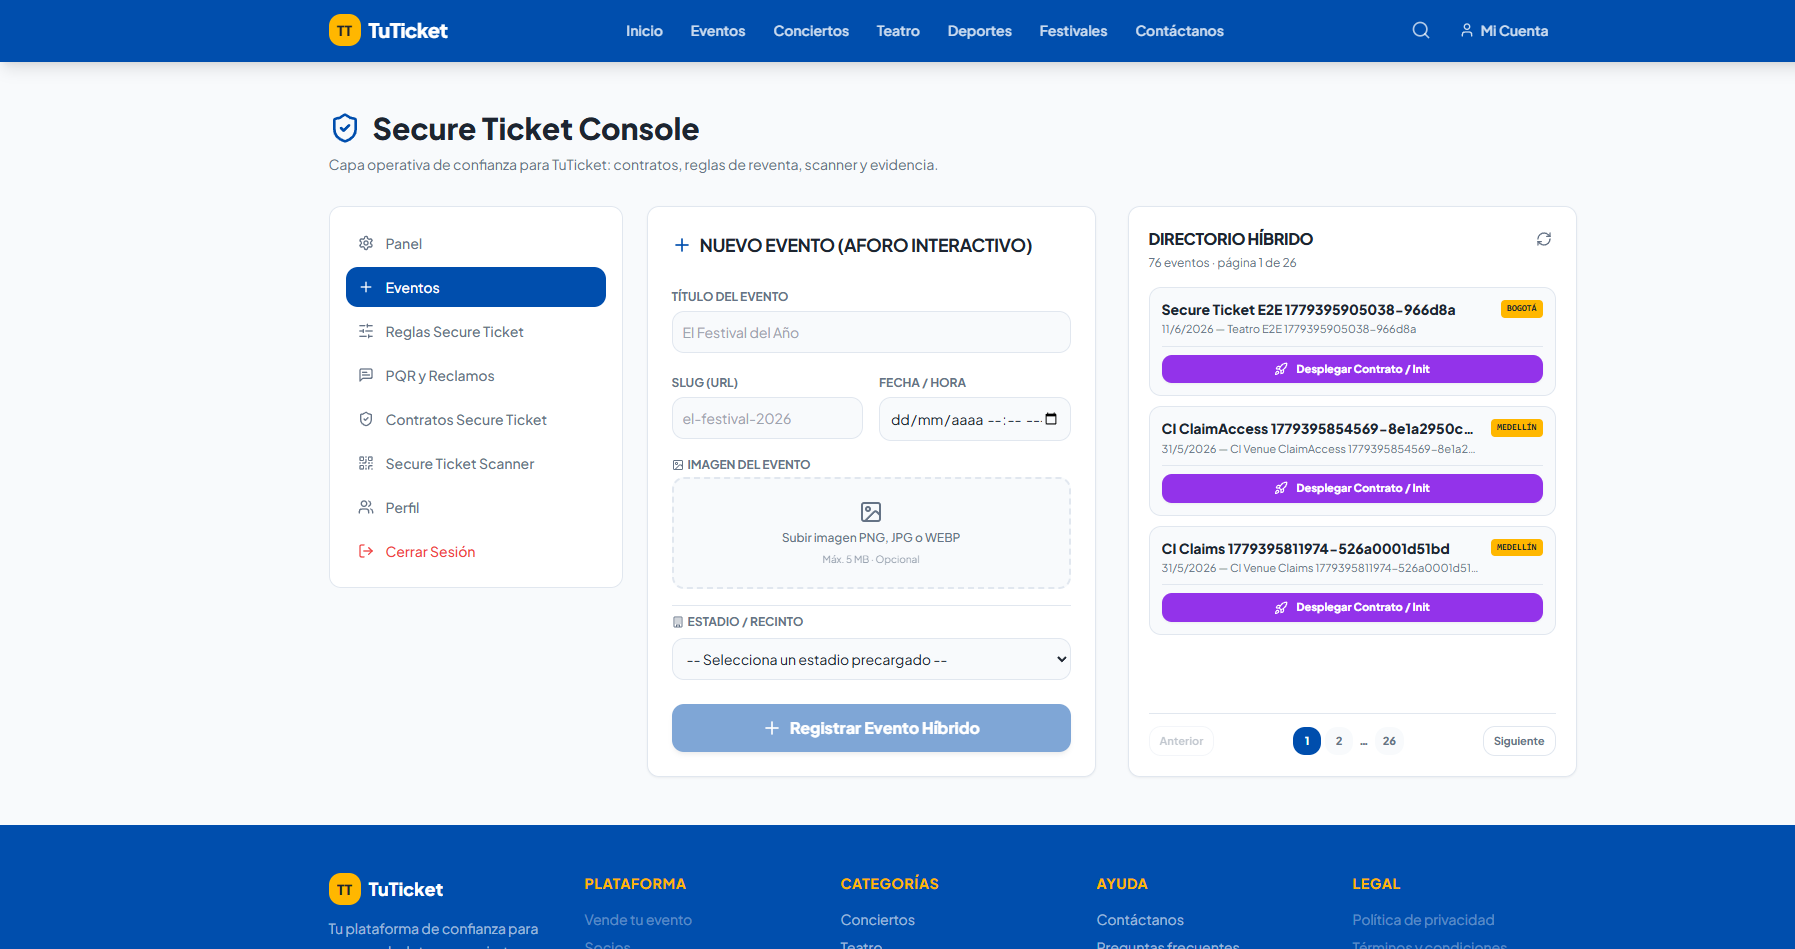
\includegraphics[width=0.85\textwidth]{Imagenes/app_01_catalogo.png}
\caption{Consola del usuario administrador: panel desde el que se despliegan los contratos Soroban para
eventos \textit{offchain} y se crean los eventos, vinculando cada evento de la pasarela tradicional con su
contrato \textit{onchain} correspondiente a través del \texttt{factory}.}
\label{fig:app-admin-consola}
\end{figure}

\begin{figure}[H]
\centering
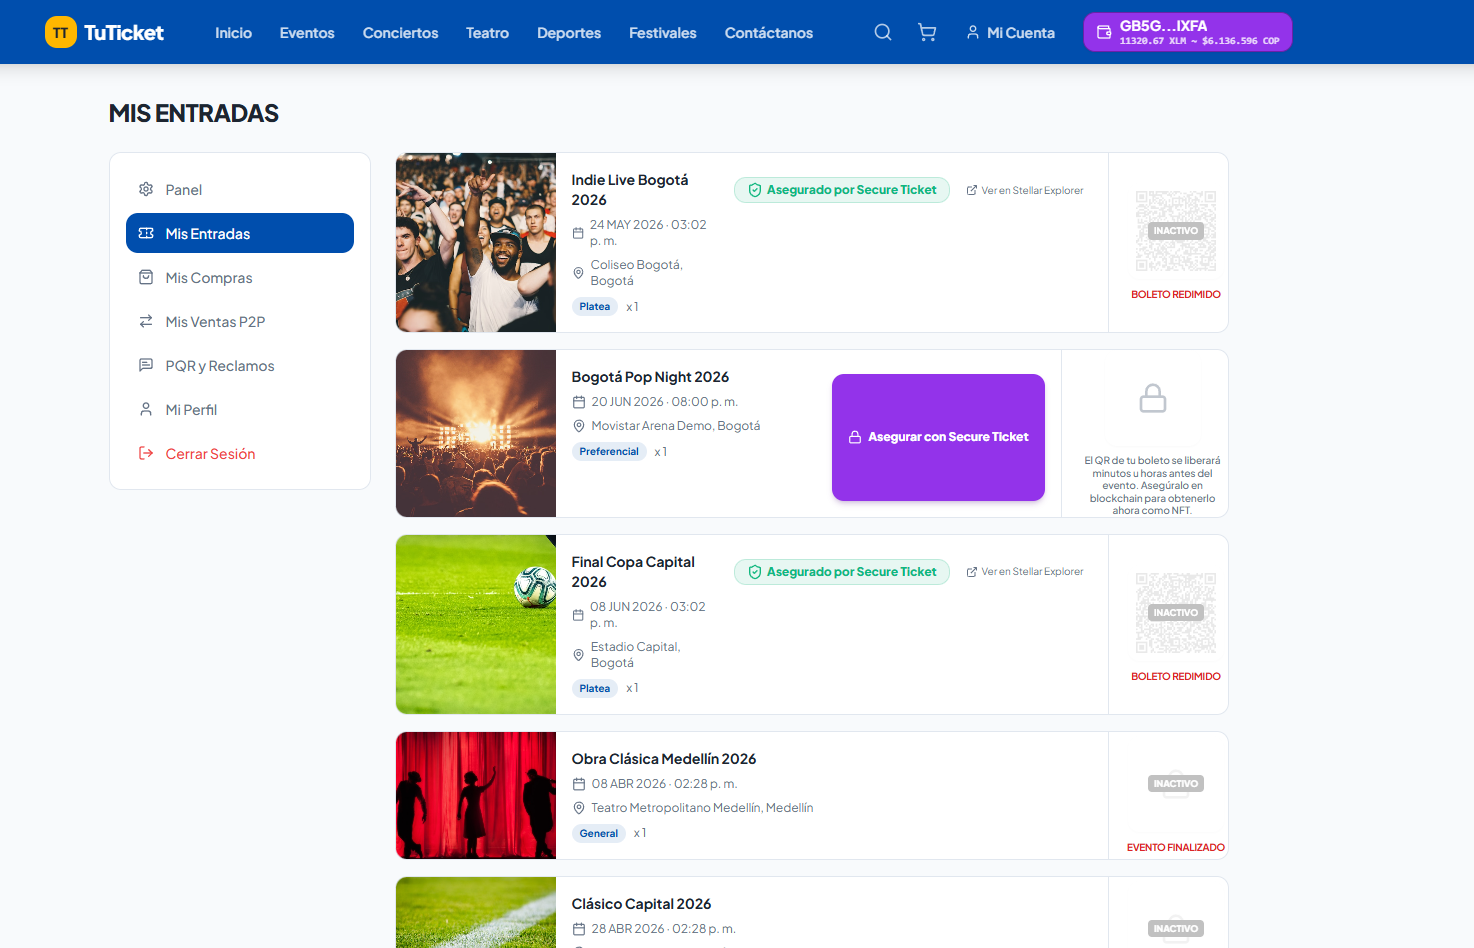
\includegraphics[width=0.85\textwidth]{Imagenes/app_07_asegurar.png}
\caption{Vista ``Mis Entradas'' del usuario final: los boletos que aún no han sido asegurados en la
blockchain se manejan de forma tradicional, por lo que el usuario debe esperar a que el organizador libere el
QR de acceso; el botón ``Asegurar en Blockchain'' permite acuñar el boleto como NFT y liberar el QR de
inmediato.}
\label{fig:app-asegurar}
\end{figure}

\begin{figure}[H]
\centering
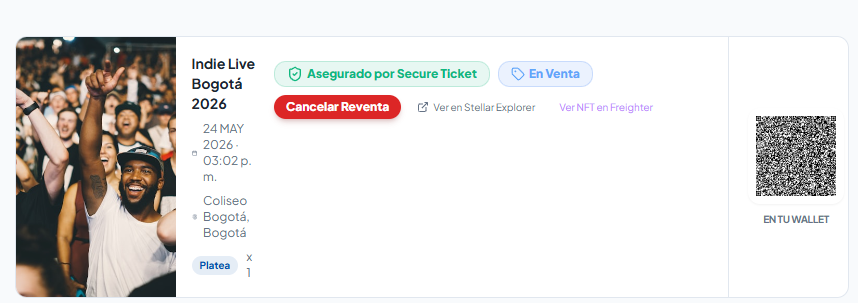
\includegraphics[width=0.85\textwidth]{Imagenes/app_08_boleto_asegurado.png}
\caption{Boleto ya asegurado en la blockchain: el QR firmado queda liberado de forma anticipada y la interfaz
expone las opciones disponibles sobre el NFT (revender en el mercado P2P, guardar el QR como
\textit{collectible} en la wallet, ver el detalle del contrato).}
\label{fig:app-asegurado}
\end{figure}

\begin{figure}[H]
\centering
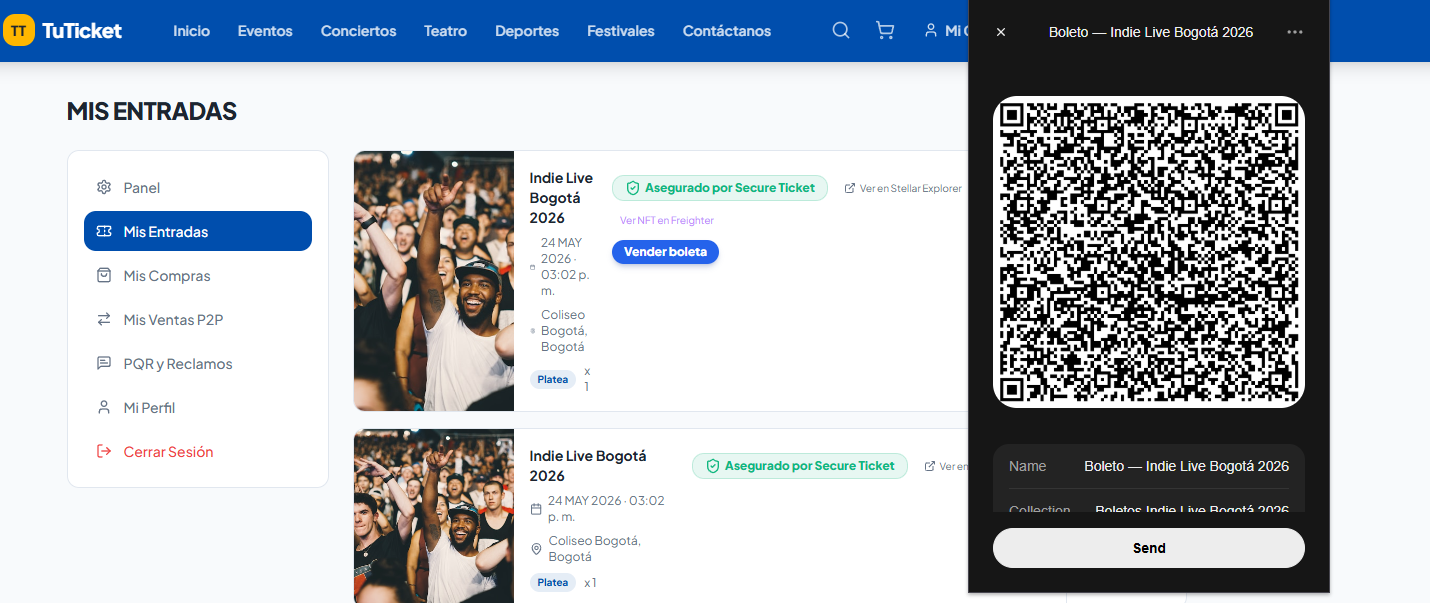
\includegraphics[width=0.85\textwidth]{Imagenes/app_04_qr_nft.png}
\caption{Una vez asegurado el boleto, el usuario puede guardar su QR como NFT \textit{collectible} dentro de
la wallet Freighter; la captura muestra cómo se visualiza el NFT del boleto dentro de la extensión.}
\label{fig:app-qr-nft}
\end{figure}

\begin{figure}[H]
\centering
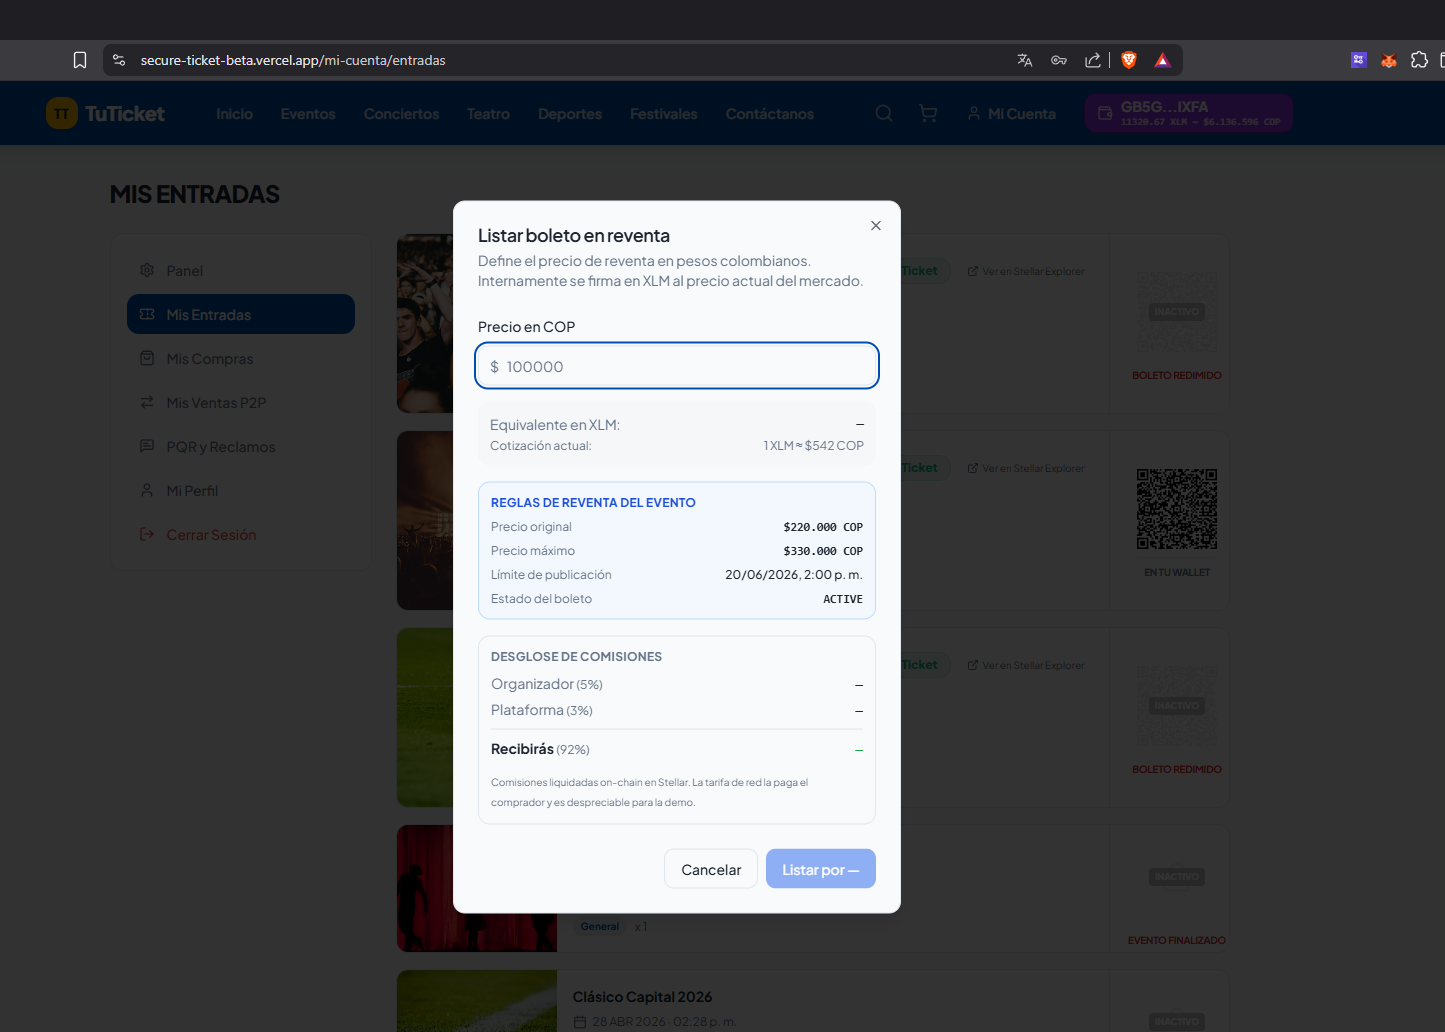
\includegraphics[width=0.85\textwidth]{Imagenes/app_02_listar_reventa.png}
\caption{Listado de un boleto para reventa: el usuario fija el precio en COP, la interfaz muestra el equivalente en XLM a la cotización actual y descompone las comisiones (5\,\% organizador, 3\,\% plataforma) junto al monto neto a recibir.}
\label{fig:app-listar}
\end{figure}

\begin{figure}[H]
\centering
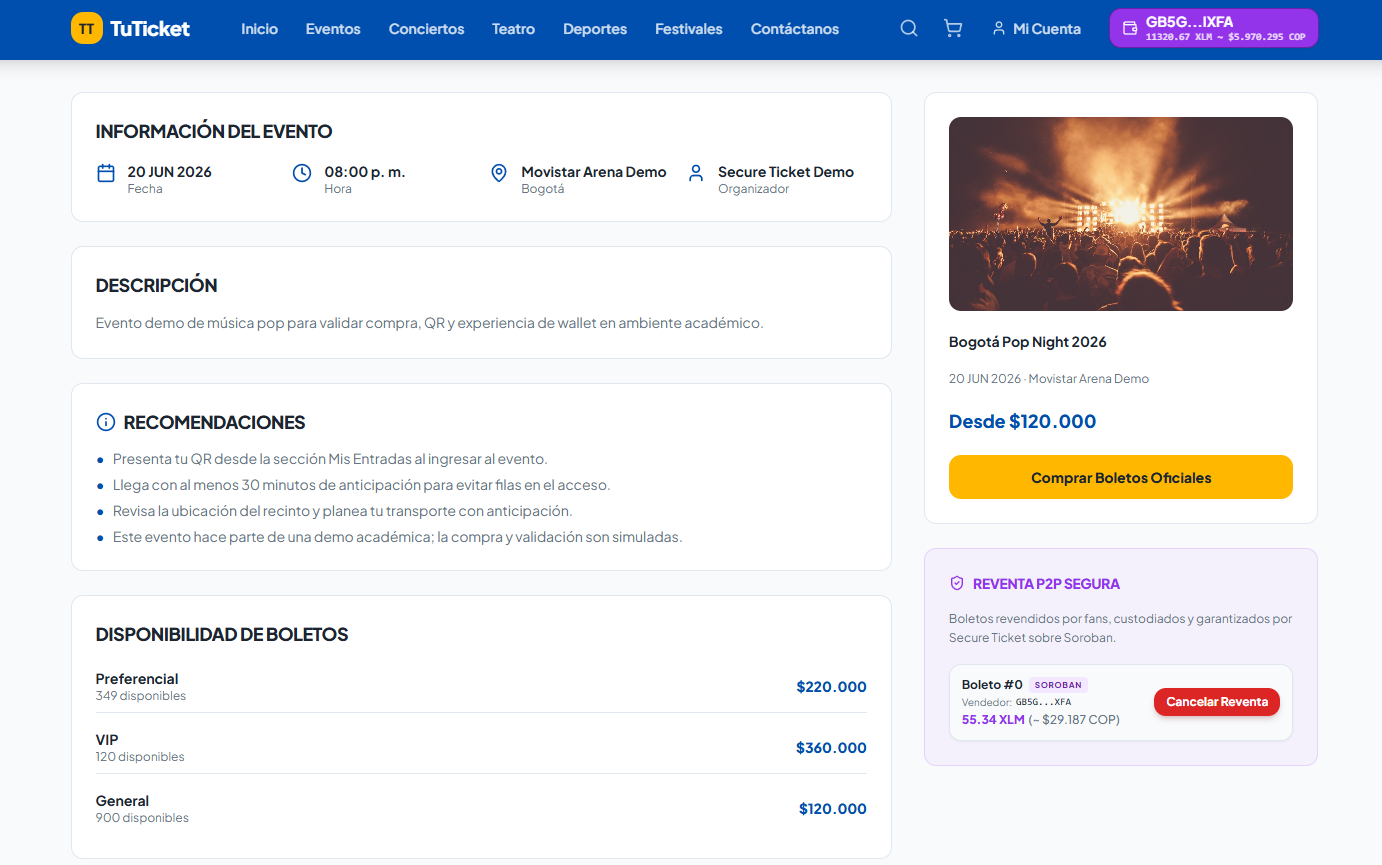
\includegraphics[width=0.85\textwidth]{Imagenes/app_09_boleta_reventa_p2p.png}
\caption{Vista pública del mercado secundario: así ve un usuario una boleta publicada en la red Stellar
disponible para compra P2P, con el precio fijado por el revendedor, el detalle del evento y el botón para
ejecutar la compra atómica contra el contrato.}
\label{fig:app-reventa-p2p}
\end{figure}

\begin{figure}[H]
\centering
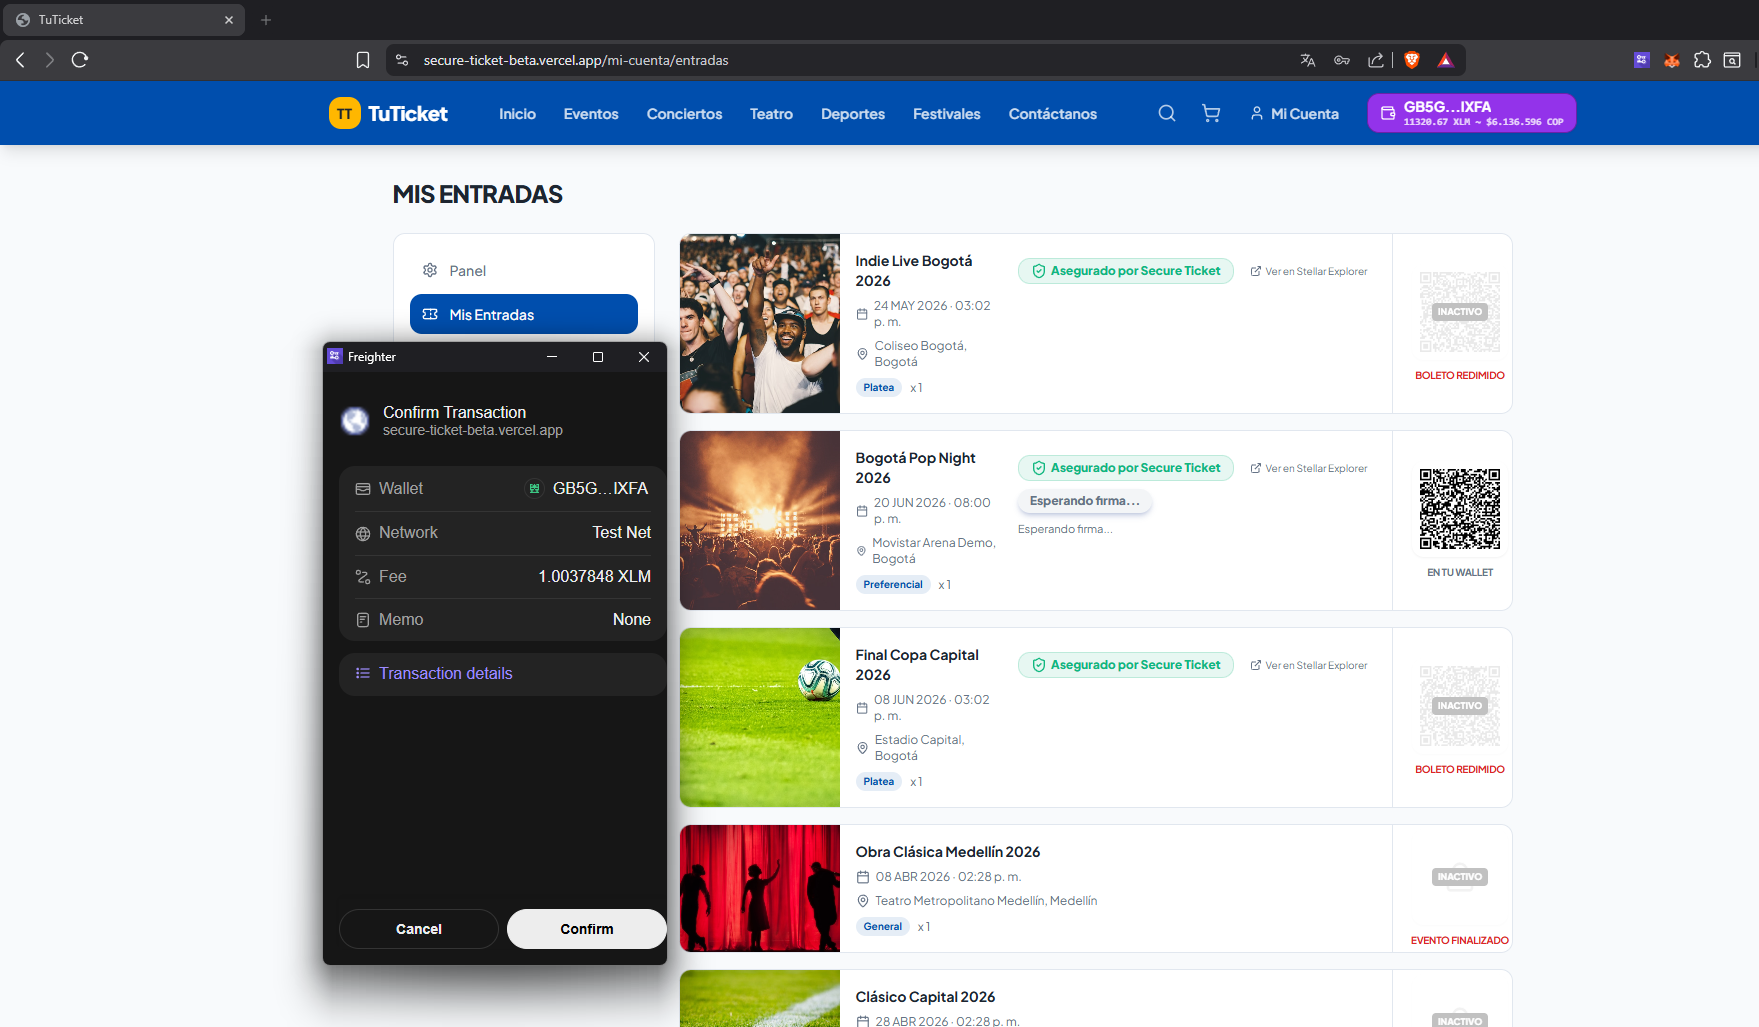
\includegraphics[width=0.85\textwidth]{Imagenes/app_03_freighter_firma.png}
\caption{Ejemplo de cómo el usuario ve en la extensión Freighter el detalle de la transacción Soroban
construida por el backend (XDR proxy) y cómo esta solicita su firma con la llave privada local; esta
confirmación se solicita tanto al publicar un boleto en reventa como al momento de comprarlo, y las llaves
privadas nunca abandonan la extensión.}
\label{fig:app-freighter}
\end{figure}

\begin{figure}[H]
\centering

\includegraphics[width=0.85\textwidth]{Imagenes/app_10_detalle_wallet.png}
\caption{Detalle de la wallet del usuario una vez vinculada su sesión con la extensión Freighter: la interfaz
muestra el saldo en XLM y su equivalente en COP a la cotización actual, integrando la información on-chain de
la cuenta con la representación monetaria local.}
\label{fig:app-wallet}
\end{figure}

\begin{figure}[H]
\centering
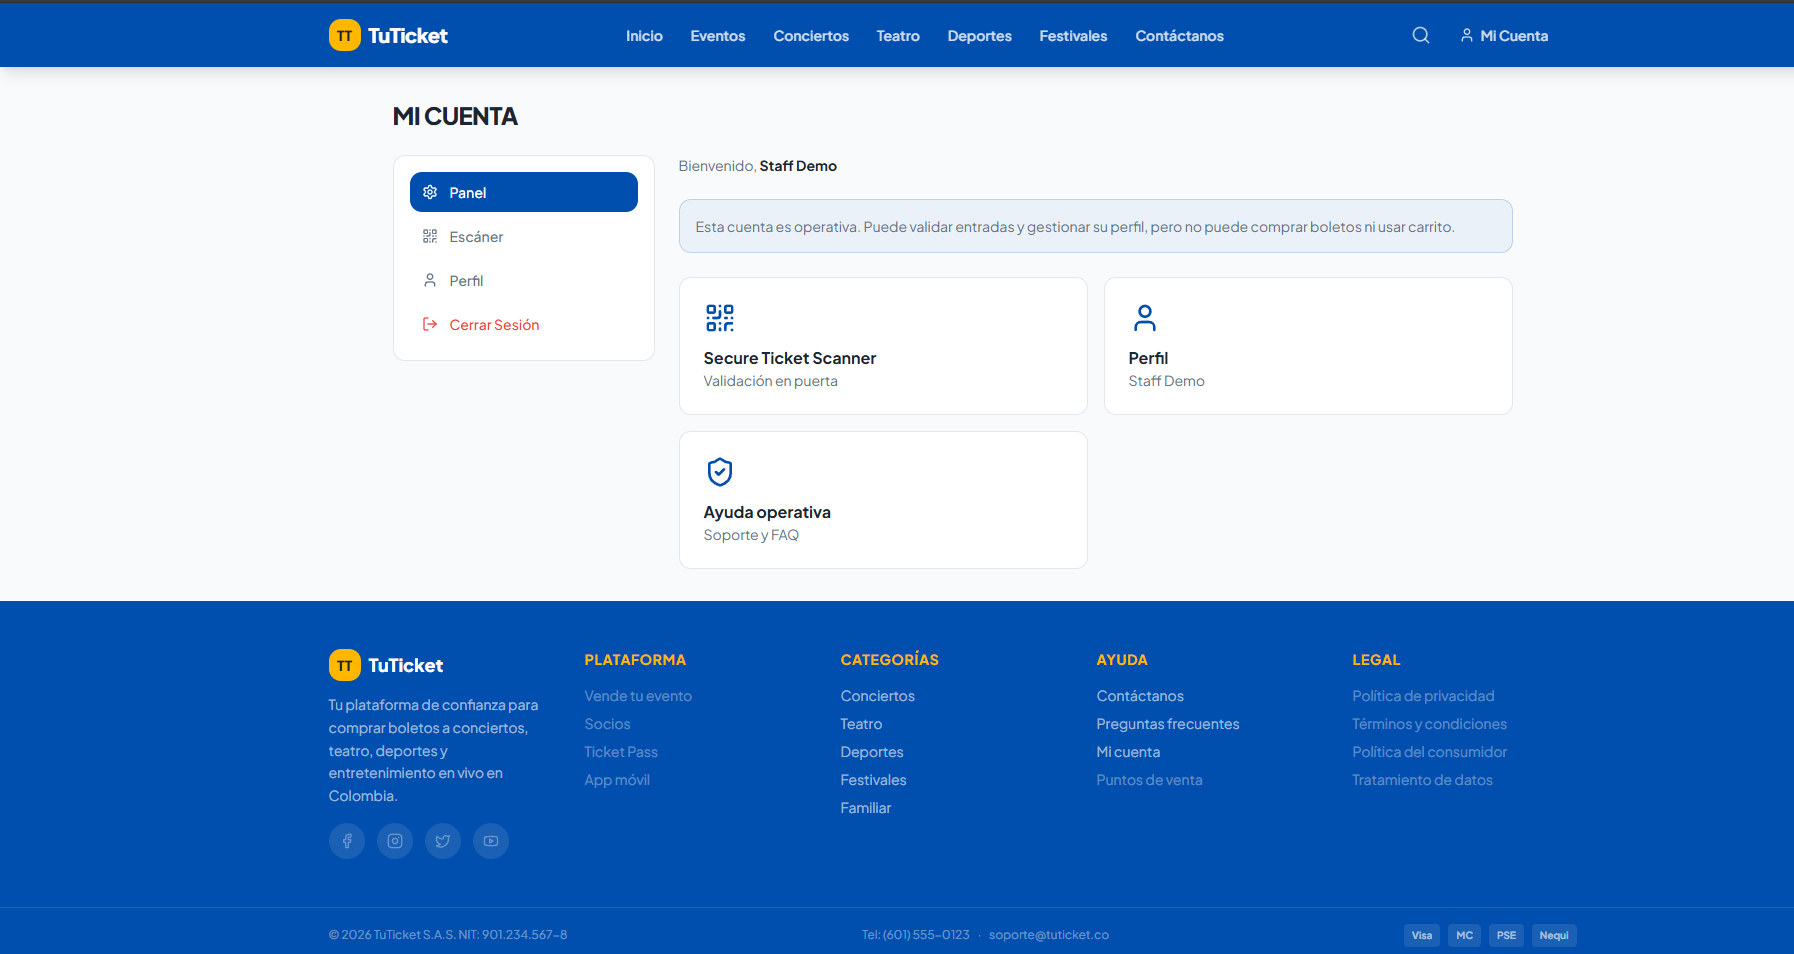
\includegraphics[width=0.85\textwidth]{Imagenes/app_05_admin_console.png}
\caption{Consola del personal de \textit{staff} (puerta de acceso): los validadores en puerta acceden a un
panel reducido cuya única funcionalidad disponible es el ``Secure Ticket Scanner'', utilizado para escanear y
validar los QR NFT presentados por los asistentes.}
\label{fig:app-staff}
\end{figure}

\begin{figure}[H]
\centering
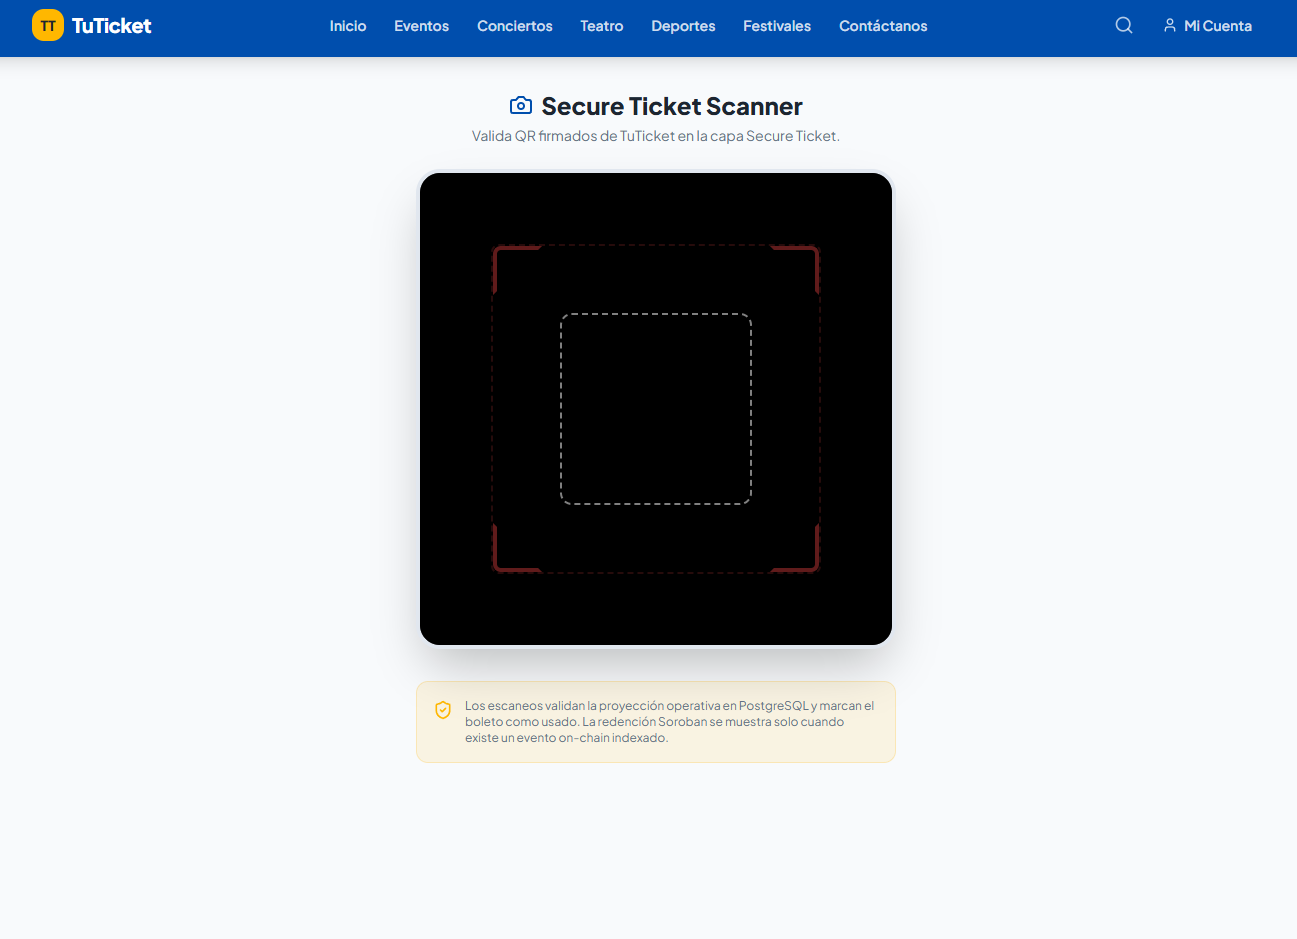
\includegraphics[width=0.85\textwidth]{Imagenes/app_06_ui_escanner.png}
\caption{Vista del \textit{Secure Ticket Scanner} tal como la observa el personal de \textit{staff} en
puerta: la cámara escanea el QR NFT del asistente y la interfaz reporta el resultado de la verificación
contra el contrato \texttt{ticket\_nft\_contract}, marcando el boleto como redimido en caso de éxito.}
\label{fig:app-scanner}
\end{figure}

Como complemento a las capturas de la aplicación, se incluyen a continuación tres vistas tomadas del
explorador público \textit{Stellar Expert}, que permiten contrastar el comportamiento de la interfaz con la
actividad efectivamente registrada en la red. Estas evidencias documentan el flujo de reventa desde la
perspectiva del ledger y verifican que las acciones del usuario se traducen en transacciones reales,
auditables por cualquier tercero.

\begin{figure}[H]
\centering
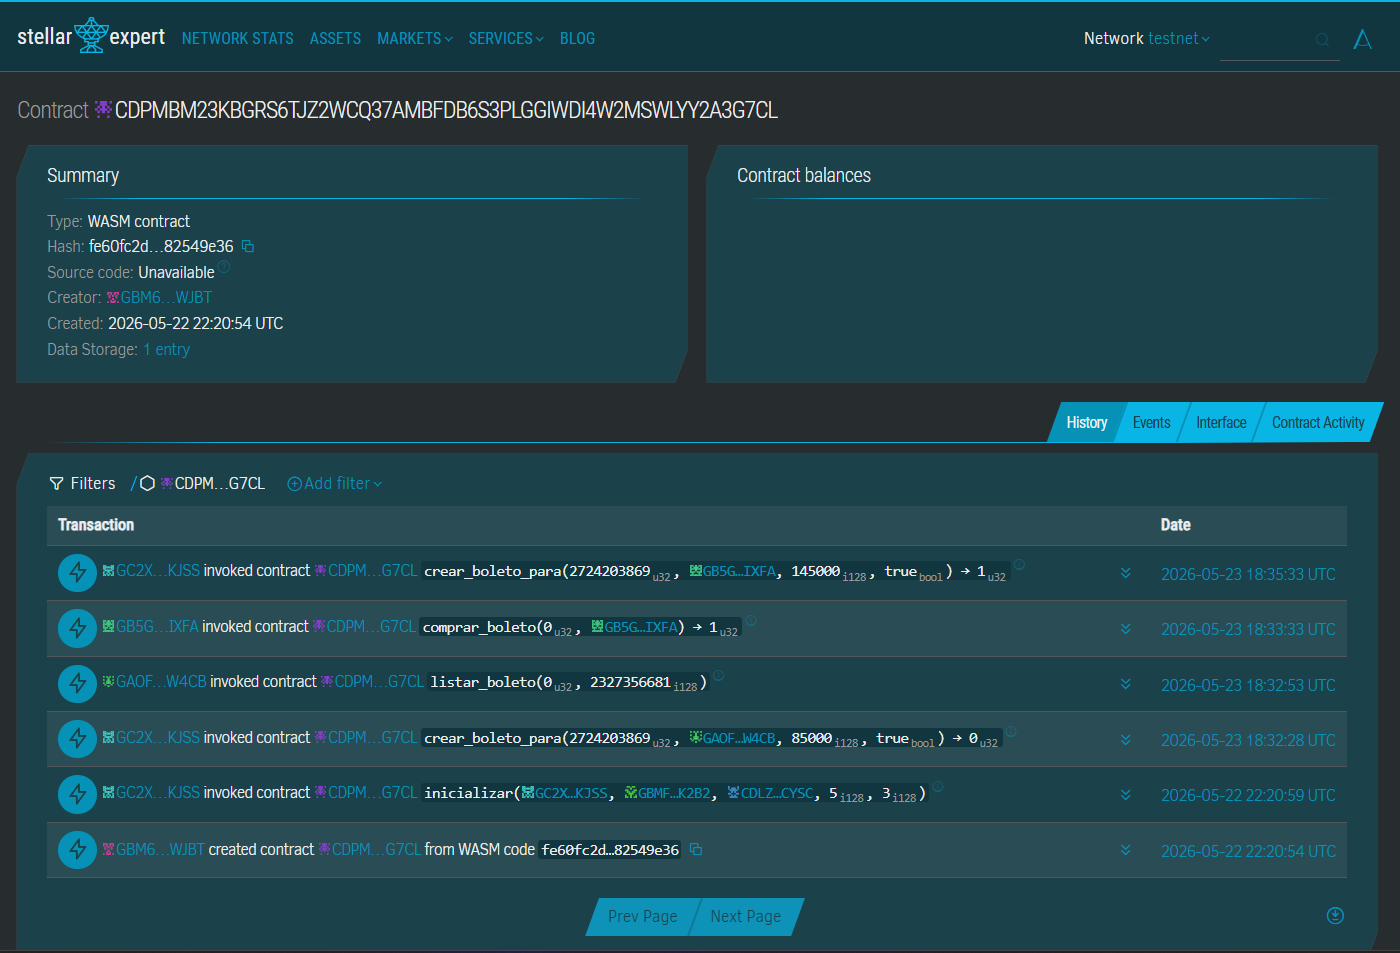
\includegraphics[width=0.85\textwidth]{Imagenes/stellar_expert_01_contrato.png}
\caption{Vista general del contrato Soroban de SecureTicket (\texttt{CDPM\ldots G7CL}) en el explorador
\textit{Stellar Expert}. El panel de resumen muestra los metadatos del contrato (\textit{hash} WASM, fecha
de despliegue, tipo de instancia) y la pestaña \textit{History} expone la lista cronológica de
invocaciones recibidas. La presencia de actividad reciente confirma que el contrato se encuentra
desplegado, accesible y operando como punto único de coordinación \textit{onchain} de los flujos de
boletería.}
\label{fig:stellar-expert-contrato}
\end{figure}

\begin{figure}[H]
\centering
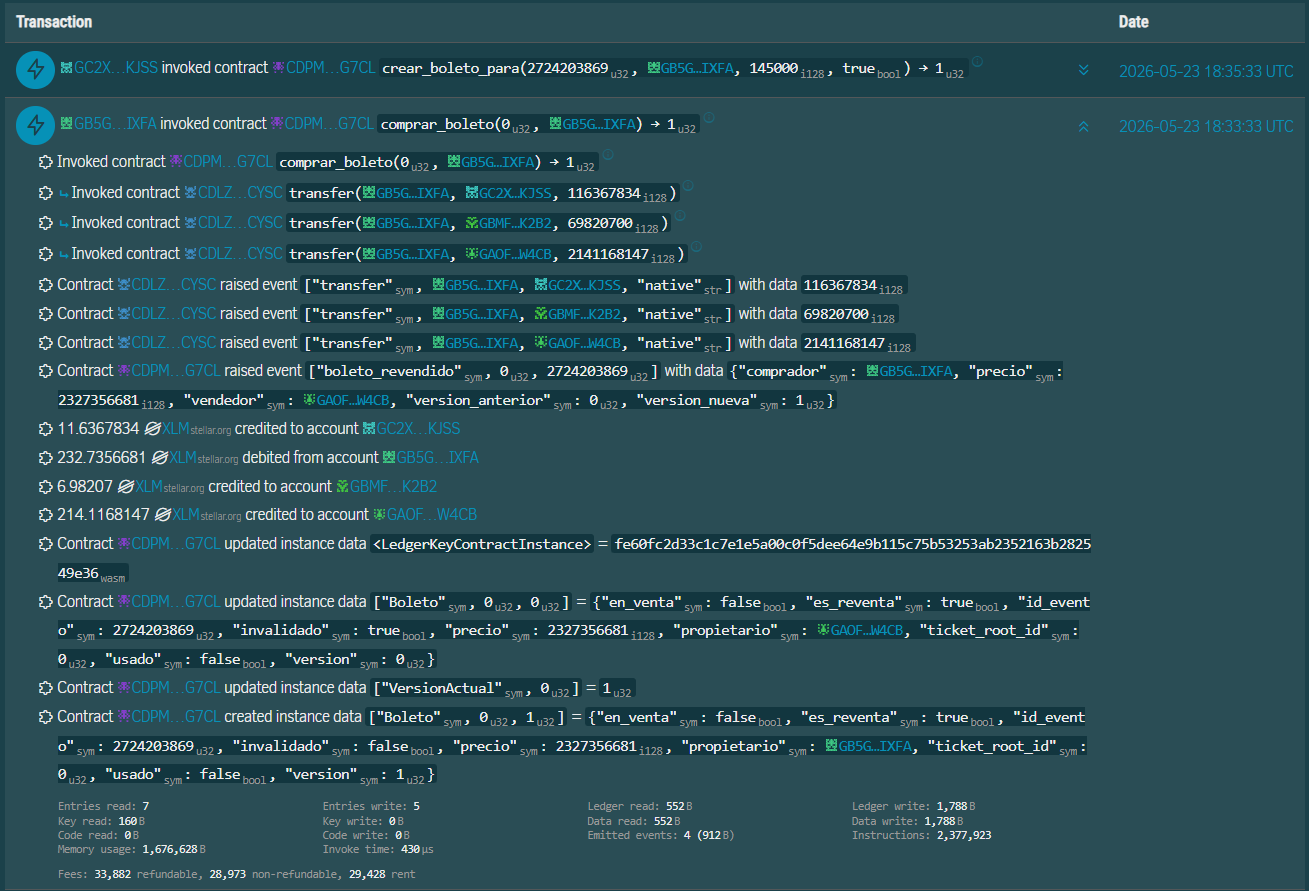
\includegraphics[width=0.85\textwidth]{Imagenes/stellar_expert_02_historial.png}
\caption{Detalle del historial de transacciones asociadas al contrato durante una sesión de reventa. Se
observa la secuencia de operaciones atómicas que componen el flujo: invocaciones a funciones del
contrato, creación y actualización de entradas \textit{instance data} (estado del boleto y contadores) y
operaciones de \textit{restore} del \textit{ledger}, propias del modelo de persistencia diferida de
Soroban. Esta traza demuestra que el cambio de propiedad de un boleto en el mercado secundario no es una
operación opaca, sino una sucesión verificable de mutaciones de estado registradas en la red Stellar.}
\label{fig:stellar-expert-historial}
\end{figure}

\begin{figure}[H]
\centering
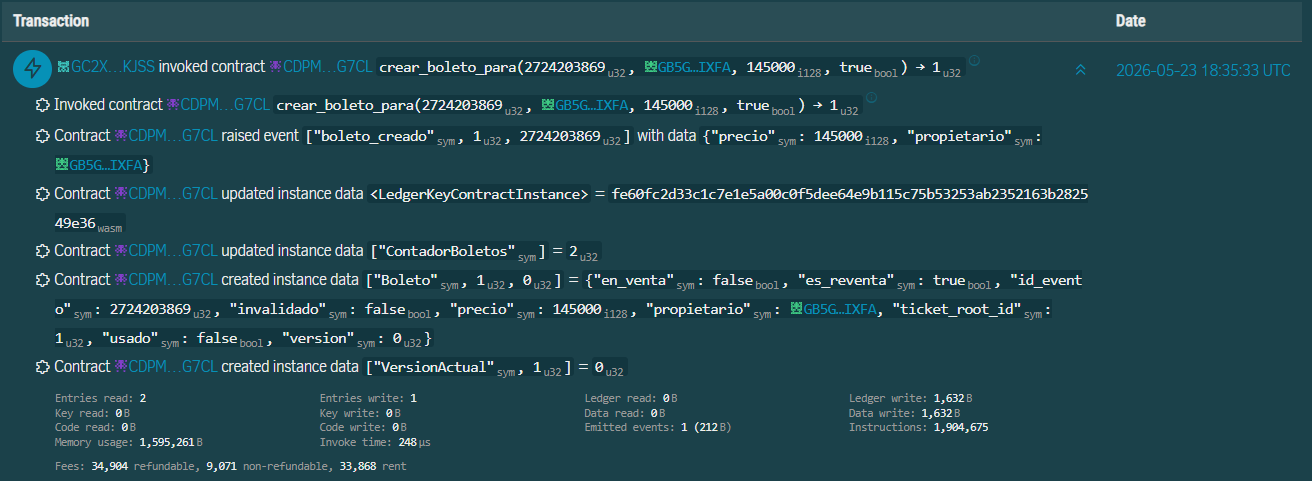
\includegraphics[width=0.95\textwidth]{Imagenes/stellar_expert_03_crear_boleto.png}
\caption{Detalle expandido de una invocación a la función \texttt{crear\_boleto\_para} ejecutada el
23 de mayo de 2026. La transacción acuña un boleto marcado como producto de reventa
(\texttt{es\_reventa\,=\,true}) y lo asigna al nuevo propietario \texttt{GB5G\ldots IXFA} por un precio
de 145\,000 \textit{stroops}, emitiendo el evento \texttt{boleto\_creado} que es consumido por el
indexador del \textit{frontend}. La captura registra además las métricas de ejecución reportadas por la
red: 248\,$\mu$s de tiempo de invocación, 1{,}9 millones de instrucciones, 1{,}6\,KB escritos en el
\textit{ledger} y comisiones del orden de 78\,000 \textit{stroops} entre porción reembolsable, no
reembolsable y \textit{rent}. Estos valores evidencian que la operación es funcionalmente correcta y
económicamente viable bajo las condiciones de la red de pruebas.}
\label{fig:stellar-expert-crear-boleto}
\end{figure}
